\documentclass[10pt]{article}
\usepackage[margin=18mm]{geometry}
\usepackage[T1]{fontenc}
\usepackage{lmodern}
\usepackage{tikz}
\usetikzlibrary{positioning,arrows.meta,fit}
\usepackage{longtable}
\usepackage{booktabs}
\usepackage{array}
\usepackage{enumitem}
\usepackage[hidelinks]{hyperref}
\setlist{nosep,leftmargin=*}
\newcommand{\code}[1]{\texttt{\detokenize{#1}}}
\newcolumntype{L}[1]{>{\raggedright\arraybackslash}p{#1}}

\title{Shared Core semantic reads over retained IR:\\base linearization, effective fields and instance slots}
\author{HyMeKo Core -- PlanOnly discovery bundle}
\date{Created-at: 2026-09-17 15:49 +02:00}

\begin{document}
\maketitle

\section*{Status and authority}
\begin{itemize}
\item \textbf{PlanOnly.} No protected Core source, dependency, fixture, lockfile or \code{CORE.YAML} item was edited.
  Implementation of step S2 requires the literal token \code{APPROVED-CORE-EDIT: ir-semantic-reads}, which has
  \emph{not} been given. The earlier \code{ir-value-updates}, \code{ir-snapshot-install} and
  \code{ir-stream-cbor-snapshot} approvals do not cover this work.
\item \textbf{ETA (after approval and decisions D1--D5).} Core S2: 3--4\,h (one module of roughly 400 LOC plus about 30 tests,
  basis: \code{value_updates.rs}, 455 LOC including tests). Query/Geometry S3: about 2\,h. Robotics S5: 2--3\,h.
  Formula S4: about 2\,h once unblocked. Simulator/XR repin S6: about 1\,h (the published Simulator catalog build took 63\,s).
\item \textbf{Scope.} Discovery of which HyMeKo authoring semantics work, which depend on the consumer, and which are
  missing. The plan proposes an additive, borrowed-IR Core API for base relations, effective fields and instance-slot
  identity, plus migration order and acceptance cases. Out of scope: simulator/XR features, benchmarks,
  deployment, push to main, parser changes, a second IR, MessagePack, and text regeneration/reparse for runtime state.
\end{itemize}

\section{Revision baseline}
Fetched 2026-09-17 15:36 +02:00 (\code{git fetch --all}); Core refetched 15:48, still 0/0. Every checkout is 0/0 against its
upstream. The Robotics and Kawamirai HTTP remotes failed authentication; their SSH \code{ls-remote} matches local HEAD.
All of these are integration feature branches, not \code{main}. This is not an ecosystem merge or release, and a
build of the full stack from a clean clone has not been demonstrated.

\begin{longtable}{L{33mm}L{52mm}L{25mm}L{55mm}}
\toprule
Checkout & Branch & HEAD & Notes\\\midrule
core & feat/ir-runtime-updates & 2c4e072 & parser pin f1162859; clean except untracked TeX byproducts\\
parser & master & be52aac & grammar surface identical to f1162859 (builder refactor only)\\
transformation & feat/robotics-authoring-integration & a0b5420 & clean\\
transformation-formula & feat/formula-nurbs & 7ef03ac & \textbf{other worker, uncommitted} (actuation, kinematic, contact, engine, visual)\\
graph & chore/published-ir-runtime & be8da9c & \\
akoire & feat/belief-planner & 2e64c4b & \\
hive & feat/lan-model-catalog & e708ff6 & \\
axon & feat/lan-ir-transport & ee6ae5d & \\
robotics & feat/robotics-belief-planner & 9ec076c & untracked \code{texput.log}\\
kawamirai / hymeko\_web / xr & feat/xr-passthrough-rendering / feat/scenario-runtime / feat/native-quest-workbench & 5d022ba / be3da44 / d674d72 & \\
simulator (xr-publish) & feat/quest-immersive-ui & 4da2729 & \code{[patch]} points at the dirty Formula worktree\\
\bottomrule
\end{longtable}
Other open items: \code{core-parser-be52aac} and \code{core_cpp} carry other-worker changes. SomaChordex is not
under Git. \code{computer-vision-modules} has no remote. \code{ecosystem.hymeko} lists 17 repositories and does
\emph{not} list \code{robotics} or \code{hystl}, even though the Robotics manifest consumes both. This is recorded as
map drift and is not fixed here.

\section{Evidence: semantics that already work}
Basis key: R = read in code; P = Core CLI probe run in this task (Core release binary rebuilt at 2c4e072); T = existing test.

\begin{longtable}{L{8mm}L{62mm}L{85mm}L{8mm}}
\toprule
\# & Capability & Location (file : symbol) and fact & Basis\\\midrule
E1 & Base references on nodes and edges & \code{parser/src/hymeko.lalrpop}: \code{BaseRef}, \code{NodeBlockStart}, \code{EdgeBlockStart}. A base is signed \code{+ - ~} or unsigned (lowered as Neutral), and carries tags and an optional value. & R\\
E2 & No template or instantiation syntax & The Description grammar has none; \code{? * ..} exist only for \code{QueryVar} and unused rules. & R\\
E3 & Bases retained, never expanded & \code{ir/lower.rs}: \code{lower_node}/\code{lower_edge} $\to$ \code{NodeRec/EdgeRec.bases: Vec<SignedRefR>} in authored order with sign/tags/weights. An edge instance does not inherit base arcs (probe p8: 1 arc). & R,P\\
E4 & Identity-preserving references & \code{resolution/resolve.rs}: \code{resolve_ref_to_declid} $\to$ \code{ValueR::Ref(DeclId)}. Lookup is lexical containment plus module-local \code{using}/import aliases. A match at more than one scope level is \code{AmbiguousRef} (p5), not shadowing. Base members are not reachable by path (p2b \code{UnresolvedRef inst.friction}). Duplicate paths are an error. & R,P\\
E5 & Diamond imports share identity & \code{module_store.rs}: \code{linked_imports} links each canonical file once. & R\\
E6 & Compile-time arithmetic & \code{resolution/const_resolve.rs}: \code{evaluate_consts}/\code{resolve_consts} handle forward refs and detect cycles, division by zero and undefined names; \code{pi}, \code{exp}. The IR stores only the folded \code{Num}. & R,P,T\\
E7 & Signed incidences with roles & \code{ArcRec.refs} holds target, sign, tags, weights and \code{direction=Unspecified}. \code{ir/incidence.rs}: \code{IncidenceIndex}, \code{IncidenceRef} give reverse navigation; Graph \code{direct_ir} uses them (Robotics A*). & R,T\\
E8 & Structural read API & \code{ir/access.rs} (total accessors); \code{canonical_hash::build_path_index} $\to$ \code{DerivedPathIndex} (path $\leftrightarrow$ DeclId). & R\\
E9 & Runtime value updates without parser & \code{module_store/execution/value_updates.rs}: \code{CompiledModel::with_value_updates} takes \code{Set/Text/Clear} on leaf Node declarations only. It is copy-on-write, keeps IDs/hierarchy/bases/index, and validates coherence and the model contract. Derived expressions are not re-evaluated. \code{ExecutionState::prepare_model_at/commit} reject stale or foreign bases. & R,T\\
E10 & Canonical CBOR plus \code{ir_stream} & \code{writers/cbor_writer/stream.rs}: \code{encode_snapshot_messages}/\code{decode_snapshot}; assembler Begin$\to$Chunk$^*\to$Commit; \code{CompiledModel::from_decoded_cbor}. HIVE \code{lan.rs} and \code{lib.rs::apply_value} use exactly these. & R,T\\
E11 & Navigation example & \code{robotics/examples/cyberdisc/navigation.hymeko}: import/\code{using}, \code{+ <isa>} classification, a 3-point hyperedge region, shared profile references, per-instance \code{state}, const arithmetic. \code{navigation.rs::NavigationView::read} feeds Graph \code{astar_berge_path} and the AKOIRE \code{PlanGate}. \code{tests/navigation.rs}: detour 4\,m$\to$8\,m through \code{ValueUpdate::Text} with no source read; a shared profile update affects every referencing region; reference rebinding; the \code{raduis_m} mutation is rejected as a missing field. & R,T\\
E12 & ArUco observation state & \code{robotics/src/perception/recording.rs}: \code{RecordingSlots} requires authored leaf slots; each capture is applied as \code{ValueUpdate}s through \code{ExecutionState}. \code{perception.rs::source} emits text only as an export projection. & R,T\\
\bottomrule
\end{longtable}

\section{Consumer-dependent semantics (present, not shared)}
\begin{longtable}{L{8mm}L{45mm}L{112mm}}
\toprule
\# & Capability & Implementations and their divergence\\\midrule
C1 & ``X is-a Y'' & Seven walks. Query \code{QueryEngine::check_inheritance}: by name, depth 8, not reflexive, tags ignored. \code{predicate_expr::decl_inherits}: visited set, reflexive. \code{rewrite/template.rs::decl_inherits_from}: depth 16. Geometry \code{check_inherits_simple}: depth 4; \code{geometry_decl}: direct bases only. WebXR \code{isa_transitive}: by DeclId, depth 1024, no deduplication. Dynamics/Optimize \code{Reader::inherits}: by name, visited set. None checks \code{<isa>} or the sign; all name-based variants are namespace-blind.\\
C2 & Field read & Direct children only in Query \code{MatchContext::resolve_field_decl}/\code{get_field_at}, Geometry \code{find_child_*} and \code{Fields} (a0b5420), Robotics \code{pipeline::Schema}, Dynamics/Optimize \code{Reader::field}, WebXR \code{attr_value}, Graph octree \code{field}. \code{MatchContext} also turns \code{ValueR::Ref} into a name string, adds an edge-base fallback and a single-child rule.\\
C3 & Inherited reference field & Geometry \code{find_inherited_ref_target} (committed): own children first, then DFS over bases, depth 4. A non-reference local \code{limit} is skipped. Used by joint limits only.\\
C4 & General inherited field (Formula) & \code{transformation-formula .../actuation.rs::Fields::child}, \textbf{uncommitted}: stack DFS in authored base order, visited set, first name match wins, sign/tags ignored, no diagnostics. The Simulator's committed manifest patches to it. Diamond case: \code{x: A, B; A: R; B: R { f }}; the DFS returns R's \code{f} before B's override.\\
\bottomrule
\end{longtable}

\section{Gaps}
\begin{enumerate}[label=G\arabic*]
\item No Core base-relation API: no selection policy, no transitive is-a by DeclId, no cycle diagnosis. \emph{Probe p1: \code{a: + <isa> b; b: + <isa> a} compiles.}
\item No Core effective-field resolution, and at least six consumer copies with contradictory order, depth and reflexivity (C1--C4).
\item No declared precedence among multiple bases and no ambiguity or diagnostic surface.
\item No owner identity for an effective value. A writer cannot tell a shared profile slot from instance state. For example, \code{sphere_impact.a} and \code{.b} both resolve \code{link_geometry} to the \code{c.sphere_body} declaration; updating that DeclId changes both.
\item No structural update. \code{with_value_updates} cannot allocate an instance slot or change bases, arcs or incidence weights (arc declarations are \code{HyperArc} and are rejected as \code{InvalidLeaf}). Mutable instance state must be authored as local slots.
\item No field-path traversal that follows references while preserving identity.
\item No field-schema validation. A misspelled override is simply a new local declaration (p2a \code{mas 4.0} compiles). This is not proposed as an automatic check.
\item Base selection is ambiguous. The language guide says \code{<isa>} marks inheritance, but corpora use untagged mixins (\code{a: link, m.impact_blue, c.sphere_body}) and namespace-like bases (\code{impact: elements, geometry, axes}).
\item Const hazards: a duplicate const silently keeps the last value (p4); a single-segment reference that matches a const name silently becomes a number (p3, \code{link -> ghost}); consts are module-local (p6); expressions keep no provenance, so there is no reactive recomputation.
\item Templates are text rendering in Query \code{rewrite}. \code{regen::emit_split_rewrite} and \code{hymeko_emitter::emit_bases} drop base sign and tags (lossy projections).
\item Ecosystem-map drift: \code{robotics} and \code{hystl} are absent from \code{ecosystem.hymeko}.
\item Publication coupling: the committed Simulator 4da2729 depends on uncommitted other-worker code in the Formula worktree.
\end{enumerate}

\section{Proposed shared Core API}
Owner: Core (capability \code{semantic_authority} and boundary \code{only_the_description_is_authoritative} in \code{ecosystem.hymeko}).
New module \code{hymeko_core/src/ir/semantics.rs} (with private submodules \code{bases}, \code{fields}); \code{ir/mod.rs} declares it.
The API is additive, read-only and derived. It borrows one \code{Ir}, is never serialized, and adds no dependency, CBOR, digest or hash change.

\begin{verbatim}
pub enum BaseSelection { All, Tagged(SymId) }
pub struct BasePolicy { pub selection: BaseSelection, pub max_depth: u16, pub max_entries: u32 }

pub struct BaseView<'ir> { /* &'ir Ir, policy, CSR linearizations */ }
impl<'ir> BaseView<'ir> {
    pub fn build(ir: &'ir Ir, policy: BasePolicy) -> Result<Self, BaseError>;
    pub fn direct_bases(&self, d: DeclId) -> impl Iterator<Item = &'ir SignedRefR> + '_;
    pub fn linearization(&self, d: DeclId) -> &[DeclId];          // starts with d
    pub fn is_a(&self, d: DeclId, class: DeclId) -> bool;          // reflexive, by DeclId
    pub fn field(&self, owner: DeclId, name: SymId) -> Option<FieldBinding<'ir>>;
    pub fn shadowed(&self, owner: DeclId, name: SymId) -> impl Iterator<Item = FieldBinding<'ir>> + '_;
    pub fn effective_fields(&self, owner: DeclId) -> impl Iterator<Item = FieldBinding<'ir>> + '_;
    pub fn path(&self, owner: DeclId, path: &[SymId]) -> Result<FieldBinding<'ir>, FieldError>;
    pub fn instance_slot(&self, owner: DeclId, name: SymId) -> Result<DeclId, SlotError>;
}
pub struct FieldBinding<'ir> {
    pub requested: DeclId,   // declaration that was asked
    pub declaration: DeclId, // slot supplying the value: the identity a ValueUpdate targets
    pub provider: DeclId,    // requested itself or a base in its linearization
    pub rank: u32,           // position of provider in the linearization (0 = local)
    pub value: Option<&'ir ValueR>,
}
impl FieldBinding<'_> {  // kind-checked, never falls back to a base
    pub fn number(&self) -> Result<f64, FieldError>;
    pub fn reference(&self) -> Result<DeclId, FieldError>;
    pub fn list(&self) -> Result<&[ValueR], FieldError>;
    pub fn text<'i>(&self, it: &'i Interner) -> Result<&'i str, FieldError>;
}
pub enum BaseError  { Cycle { path: Vec<DeclId> }, InconsistentOrder { declaration: DeclId },
                      DanglingBase { declaration: DeclId, target: DeclId }, LimitExceeded }
pub enum FieldError { Missing { owner: DeclId, name: SymId },
                      WrongKind { declaration: DeclId, expected: ValueKind, found: Option<ValueKind> },
                      ReferenceCycle { at: DeclId }, PathLimit }
pub enum SlotError  { Missing, NotLeaf { declaration: DeclId },
                      Inherited { declaration: DeclId, provider: DeclId } }
\end{verbatim}

\subsection*{Normative rules}
\begin{enumerate}[label=R\arabic*]
\item \textbf{Base selection} is an explicit policy that becomes part of every result. \code{All} takes every base reference and preserves sign and tags without filtering, which matches the behavior of all existing consumers. \code{Tagged(isa)} takes only bases carrying that tag. There is no hidden default (decision D1).
\item \textbf{Multiple inheritance order} is the C3 linearization over selected bases in authored order:
  $L(d)=d+\mathrm{merge}(L(b_1),\dots,L(b_n),[b_1..b_n])$. It is deterministic, puts a diamond ancestor after all its descendants, and fails closed with \code{InconsistentOrder}.
  Corpus check: \code{sphere_impact.a} gives $[a, link, meta\_element, impact\_blue, sphere\_body, neutral, material]$, so \code{color} still comes from \code{impact_blue}, identical to today's Formula result.
\item \textbf{Cycles} under the selected policy are detected at build time (DFS colouring) and returned as \code{BaseError::Cycle} with the DeclId path, and the whole view is refused. Compilation stays unchanged. Depth and entry limits return typed errors, never panics.
\item \textbf{Field lookup} is by \code{SymId} among the children of each provider in linearization order. The first provider that declares the name wins, based on presence: a local \code{mass;} or \code{mass {}} shadows with \code{value=None} and does not fall back. A local block replaces an inherited block as a whole (no deep merge). A wrong-kind local value yields \code{FieldError::WrongKind}, never the base value. \code{shadowed} exposes the hidden providers for diagnostics. Incomparable providers are ordered by C3, not rejected, because strict rejection would break \code{sphere_impact} (\code{impact_blue} vs \code{neutral}).
\item \textbf{Nested inherited blocks} keep the provider's identity. \code{path(a,[link_geometry,dimension])} resolves inside the \code{c.sphere_body.link_geometry} declaration, using that block's own linearization. The instance gets no private copy.
\item \textbf{References}: a stored \code{ValueR::Ref(DeclId)} is returned unchanged and is not retargeted to same-named instance declarations. \code{path} follows a reference only on intermediate segments; the terminal segment returns the binding that holds the reference. A reference cycle inside a path is a typed error.
\item \textbf{Instance state}: \code{instance_slot} succeeds only for a local leaf Node. An inherited effective binding returns \code{SlotError::Inherited}. Producers of observation or belief state (Robotics perception, AKOIRE domain adapters, HIVE clients) obtain slots through it. A shared-profile edit names the profile declaration explicitly.
\item \textbf{Validity after changes}: linearizations and binding DeclIds depend only on hierarchy, names and bases, all of which \code{with_value_updates} preserves (E9). Values are read from the borrowed \code{Ir}. Version 1 rebuilds the view for each \code{ExecutionSnapshot}; no cache is added without an explicit measurement request. Rebinding a reference changes \code{path} results on the successor only. Recompilation or snapshot installation requires a rebuild, and the borrow lifetime prevents mixing IRs.
\item \textbf{Non-goals}: no schema validation, default expansion, materialization, text generation or expression recomputation, and no change to compilation, CBOR, \code{ir_stream}, V1 hash or semantic digest.
\item \textbf{Portability}: \code{Vec}/slice data only, no filesystem, thread or clock use, no rayon, so it targets native and \code{wasm32}.
\end{enumerate}

\subsection*{Rejected alternatives}
\begin{itemize}
\item A shared helper inside Transformation/Query: Query is not the semantic owner, and Robotics, AKOIRE and HIVE must not depend on Transformation for meaning.
\item Expanding inherited fields into the IR during lowering: it changes IR, CBOR and digests, destroys shared-profile identity, and contradicts the authoring contract's sharing principle.
\item Formula DFS order: the diamond counterexample in C4.
\item Strict ambiguity errors, or an \code{<isa>}-only default: both break the existing Simulator data.
\end{itemize}

\section{Migration order (provider $\to$ consumer)}
\begin{enumerate}[label=S\arabic*]
\setcounter{enumi}{-1}
\item Done in this task: discovery, this bundle and the local report. No source change.
\item User decisions D1--D5 (below). Approval token for S2.
\item \textbf{Core}: implement the module, unit tests in the module, integration test \code{hymeko_core/tests/semantic_reads.rs} (inline \code{MemProvider} sources; \code{data/**} is locked), \code{SYMBOLS.md}, approval record in \code{CORE.YAML}, correctness gates A1--A13. Branch from freshly fetched Core according to D3.
\item \textbf{Transformation primary}: add \code{Predicate::isa(DeclId)} backed by \code{BaseView}; keep the name-based predicate with documented limits; add an effective-field mode to \code{MatchContext}; replace \code{find_inherited_ref_target} and \code{check_inherits_simple}. Pin the Core revision. Gates A14--A15.
\item \textbf{Formula worktree}: only after the other worker publishes or hands over. Replace \code{Fields::child} with \code{BaseView::field}. Gate A16 (differential).
\item \textbf{Robotics}: \code{pipeline::Schema} delegates to \code{BaseView}; navigation profile defaults and the camera-recording marker profile are refactored only with tests; recording acquires slots via \code{instance_slot}. Gates A17--A18.
\item \textbf{Simulator/XR/Web}: repin the published Geometry/Query revision, remove the dirty path patch, rerun existing catalog/robot tests. AKOIRE, HIVE, Axon, Graph, Kawamirai: no API change.
\end{enumerate}

\section{Acceptance cases (correctness only; no benchmark)}
\begin{longtable}{L{8mm}L{150mm}}
\toprule
A1 & Diamond \code{x: A, B; A: R; B: R}; \code{f} authored on R and B $\Rightarrow$ linearization $[x,A,B,R]$, provider B (discriminates C3 from the Formula DFS).\\
A2 & \code{X: A, B; Y: B, A; Z: X, Y} $\Rightarrow$ \code{InconsistentOrder}.\\
A3 & Probe p1 base cycle $\Rightarrow$ \code{BaseError::Cycle [a,b]}; the same source still compiles.\\
A4 & Unsigned, \code{-}, \code{~ <role>} and \code{+ <isa>} bases under \code{All} and \code{Tagged(isa)}: \code{is_a} as specified; sign and tags preserved in \code{direct_bases}.\\
A5 & Local override value; valueless local shadows (\code{None}); local block replaces inherited block; wrong kind $\Rightarrow$ \code{WrongKind}, and \code{shadowed} lists the base.\\
A6 & Misspelled local \code{mas} $\Rightarrow$ \code{field(mass)} returns the inherited provider, no error (documents the absence of schema validation).\\
A7 & \code{path(navigation,[regions,central,clearance,radius_m])}.declaration $=$ DeclId of \code{profiles.narrow.radius_m}; an inherited reference is not retargeted; a reference cycle gives a typed error.\\
A8 & Instance isolation: two instances with a shared base \code{state} $\Rightarrow$ \code{instance_slot} gives \code{Inherited}; with local slots the DeclIds are distinct; a \code{ValueUpdate} on inst1 leaves inst2 and the profile unchanged; a profile update changes every non-overriding inheritor; the nested shared block reports the mixin as provider.\\
A9 & View on base vs \code{with_value_updates} successor: identical linearizations and binding DeclIds; reference rebinding changes \code{path} on the successor only; the old view is unchanged.\\
A10 & \code{encode_compiled}$\to$\code{decode}$\to$\code{from_decoded_cbor} and \code{encode_snapshot_messages}$\to$\code{decode_snapshot} (Begin/Chunk/Commit): identical linearizations, bindings and values.\\
A11 & Counted parser: no parser call during build, reads or updates.\\
A12 & Malformed IR (dangling base, oversize depth) $\Rightarrow$ typed errors, no panic.\\
A13 & \code{cargo check -p hymeko_core --target wasm32-unknown-unknown --locked} and the existing \code{hymeko_web} wasm document check.\\
A14 & Query differential: \code{Predicate::inherits(name)} vs \code{BaseView::is_a} on Transformation fixtures with unique names; a name-collision fixture documents the difference.\\
A15 & Geometry \code{per_joint_limits_resolved_through_the_limit_ref} unchanged with the Core resolver.\\
A16 & Formula \code{Fields::child} vs \code{BaseView::field} on \code{meta_contact}, \code{meta_materials}, \code{sphere_impact}, \code{contact_cycle}, \code{contact_probe}: identical effective values; Simulator \code{ll_sphere_impact} and \code{tests/catalog.rs} unchanged.\\
A17 & Robotics navigation with a profile default plus override: routes 4\,m and 8\,m unchanged, provider read counts unchanged, \code{regions.*.state} gives \code{instance_slot} Ok, \code{raduis_m} still rejected.\\
A18 & Robotics recording: a marker whose \code{state} is inherited from a profile fails closed via \code{instance_slot}.\\
\bottomrule
\end{longtable}

\section{Interface changes, protected items, budget, rollback}
\begin{itemize}
\item Additive public API only; no existing signature, wire format, hash or digest changes; no dependency change.
\item \code{CORE.YAML} items touched in S2: \code{hymeko_core/src/ir/mod.rs}, new \code{hymeko_core/src/ir/semantics*.rs} (lockdown \code{full}) $\Rightarrow$ approval required. \code{hymeko_core/tests/**} is allowlisted.
\item Performance: not measured (no authorization). Design bound: build $O(D+\sum|L(d)|)$ under explicit limits; a field read is $O(|L(d)|\cdot\mathrm{children})$. It is rebuilt per snapshot at Robotics input limits (4096 declarations).
\item Rollback: additive module; consumers stay pinned to earlier revisions; revert per repository in consumer $\to$ provider order.
\end{itemize}

\section{Risks}
\begin{itemize}
\item DFS$\to$C3 changes diamond results (A1, A16 detect it); namespace-like untagged bases create pseudo-fields under \code{All}.
\item Name-based Query predicates stay namespace-blind until migrated; the WebXR walk has no deduplication.
\item Formula ownership: editing or committing another worker's uncommitted \code{Fields::child} is out of scope.
\item Writers that update a shared provider by mistake: mitigated only when they adopt \code{instance_slot} (A8, A18).
\item Const diagnostics (G9) would change compile behavior and need a separate decision.
\end{itemize}

\section{Open decisions for the user}
\begin{enumerate}[label=D\arabic*]
\item Base selection per consumer: \code{All} (compatible with the current corpus) vs \code{Tagged(isa)} (as written in the language guide), and whether untagged namespace bases should be re-authored.
\item Multiple-inheritance order: C3 (recommended) vs the current DFS.
\item Core approval token \code{APPROVED-CORE-EDIT: ir-semantic-reads}, and the target branch/base for S2.
\item Coordination of the Formula worktree owner, the \code{core-parser-be52aac} and \code{core_cpp} work, the SomaChordex repository address and the \code{computer-vision-modules} remote.
\item Whether G9 const diagnostics and G11 map drift become separate owner tasks.
\end{enumerate}

\begin{figure}[h]
\centering
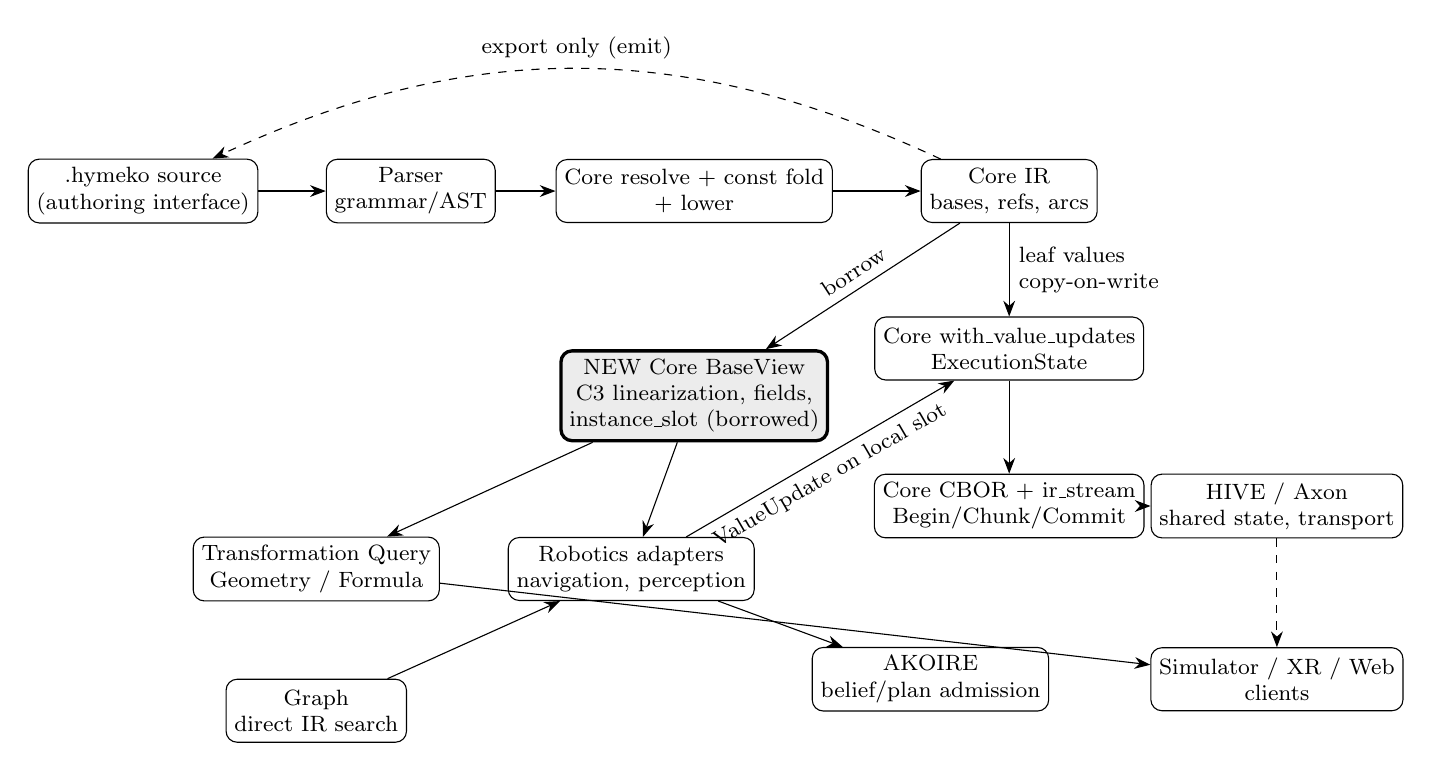
\begin{tikzpicture}[
  font=\footnotesize,
  box/.style={draw, rounded corners, align=center, minimum height=8mm, inner sep=3pt},
  new/.style={box, very thick, fill=gray!15},
  arr/.style={-{Stealth[length=2mm]}},
  dashedarr/.style={-{Stealth[length=2mm]}, dashed}
]
% Authoring and canonical compile
\node[box] (src) at (0,0) {.hymeko source\\(authoring interface)};
\node[box] (parser) at (3.4,0) {Parser\\grammar/AST};
\node[box] (lower) at (7.0,0) {Core resolve + const fold\\+ lower};
\node[box] (ir) at (11.0,0) {Core IR\\bases, refs, arcs};

% Runtime state
\node[box] (upd) at (11.0,-2.0) {Core with\_value\_updates\\ExecutionState};
\node[box] (cbor) at (11.0,-4.0) {Core CBOR + ir\_stream\\Begin/Chunk/Commit};
\node[box] (hive) at (14.4,-4.0) {HIVE / Axon\\shared state, transport};

% New semantic view
\node[new] (view) at (7.0,-2.6) {NEW Core BaseView\\C3 linearization, fields,\\instance\_slot (borrowed)};

% Consumers
\node[box] (query) at (2.2,-4.8) {Transformation Query\\Geometry / Formula};
\node[box] (rob) at (6.2,-4.8) {Robotics adapters\\navigation, perception};
\node[box] (ako) at (10.0,-6.2) {AKOIRE\\belief/plan admission};
\node[box] (graph) at (2.2,-6.6) {Graph\\direct IR search};
\node[box] (clients) at (14.4,-6.2) {Simulator / XR / Web\\clients};

\draw[arr] (src) -- (parser);
\draw[arr] (parser) -- (lower);
\draw[arr] (lower) -- (ir);
\draw[arr] (ir) -- node[right,align=left]{leaf values\\copy-on-write} (upd);
\draw[arr] (upd) -- (cbor);
\draw[arr] (cbor) -- (hive);
\draw[arr] (ir) -- node[above,sloped]{borrow} (view);
\draw[arr] (view) -- (query);
\draw[arr] (view) -- (rob);
\draw[arr] (rob) -- node[below,sloped]{ValueUpdate on local slot} (upd);
\draw[arr] (rob) -- (ako);
\draw[arr] (graph) -- (rob);
\draw[arr] (query) -- (clients);
\draw[dashedarr] (hive) -- (clients);
\draw[dashedarr] (ir) to[bend right=25] node[above]{export only (emit)} (src);
\end{tikzpicture}

\caption{Ownership and data flow; the only new element is the Core \code{BaseView}.}
\end{figure}

\end{document}
